\section{Background}
\label{sec:background}

\gls{nso} foundations can be rooted back to three enabling technologies, namely Cloud Computing, Software Defined Networking, and Network Function Virtualization. This section presents a brief overview of these topics, as well as an introduction to the historical background and definitions of term ``orchestration''.

\begin{figure*}[th]
  \centering
  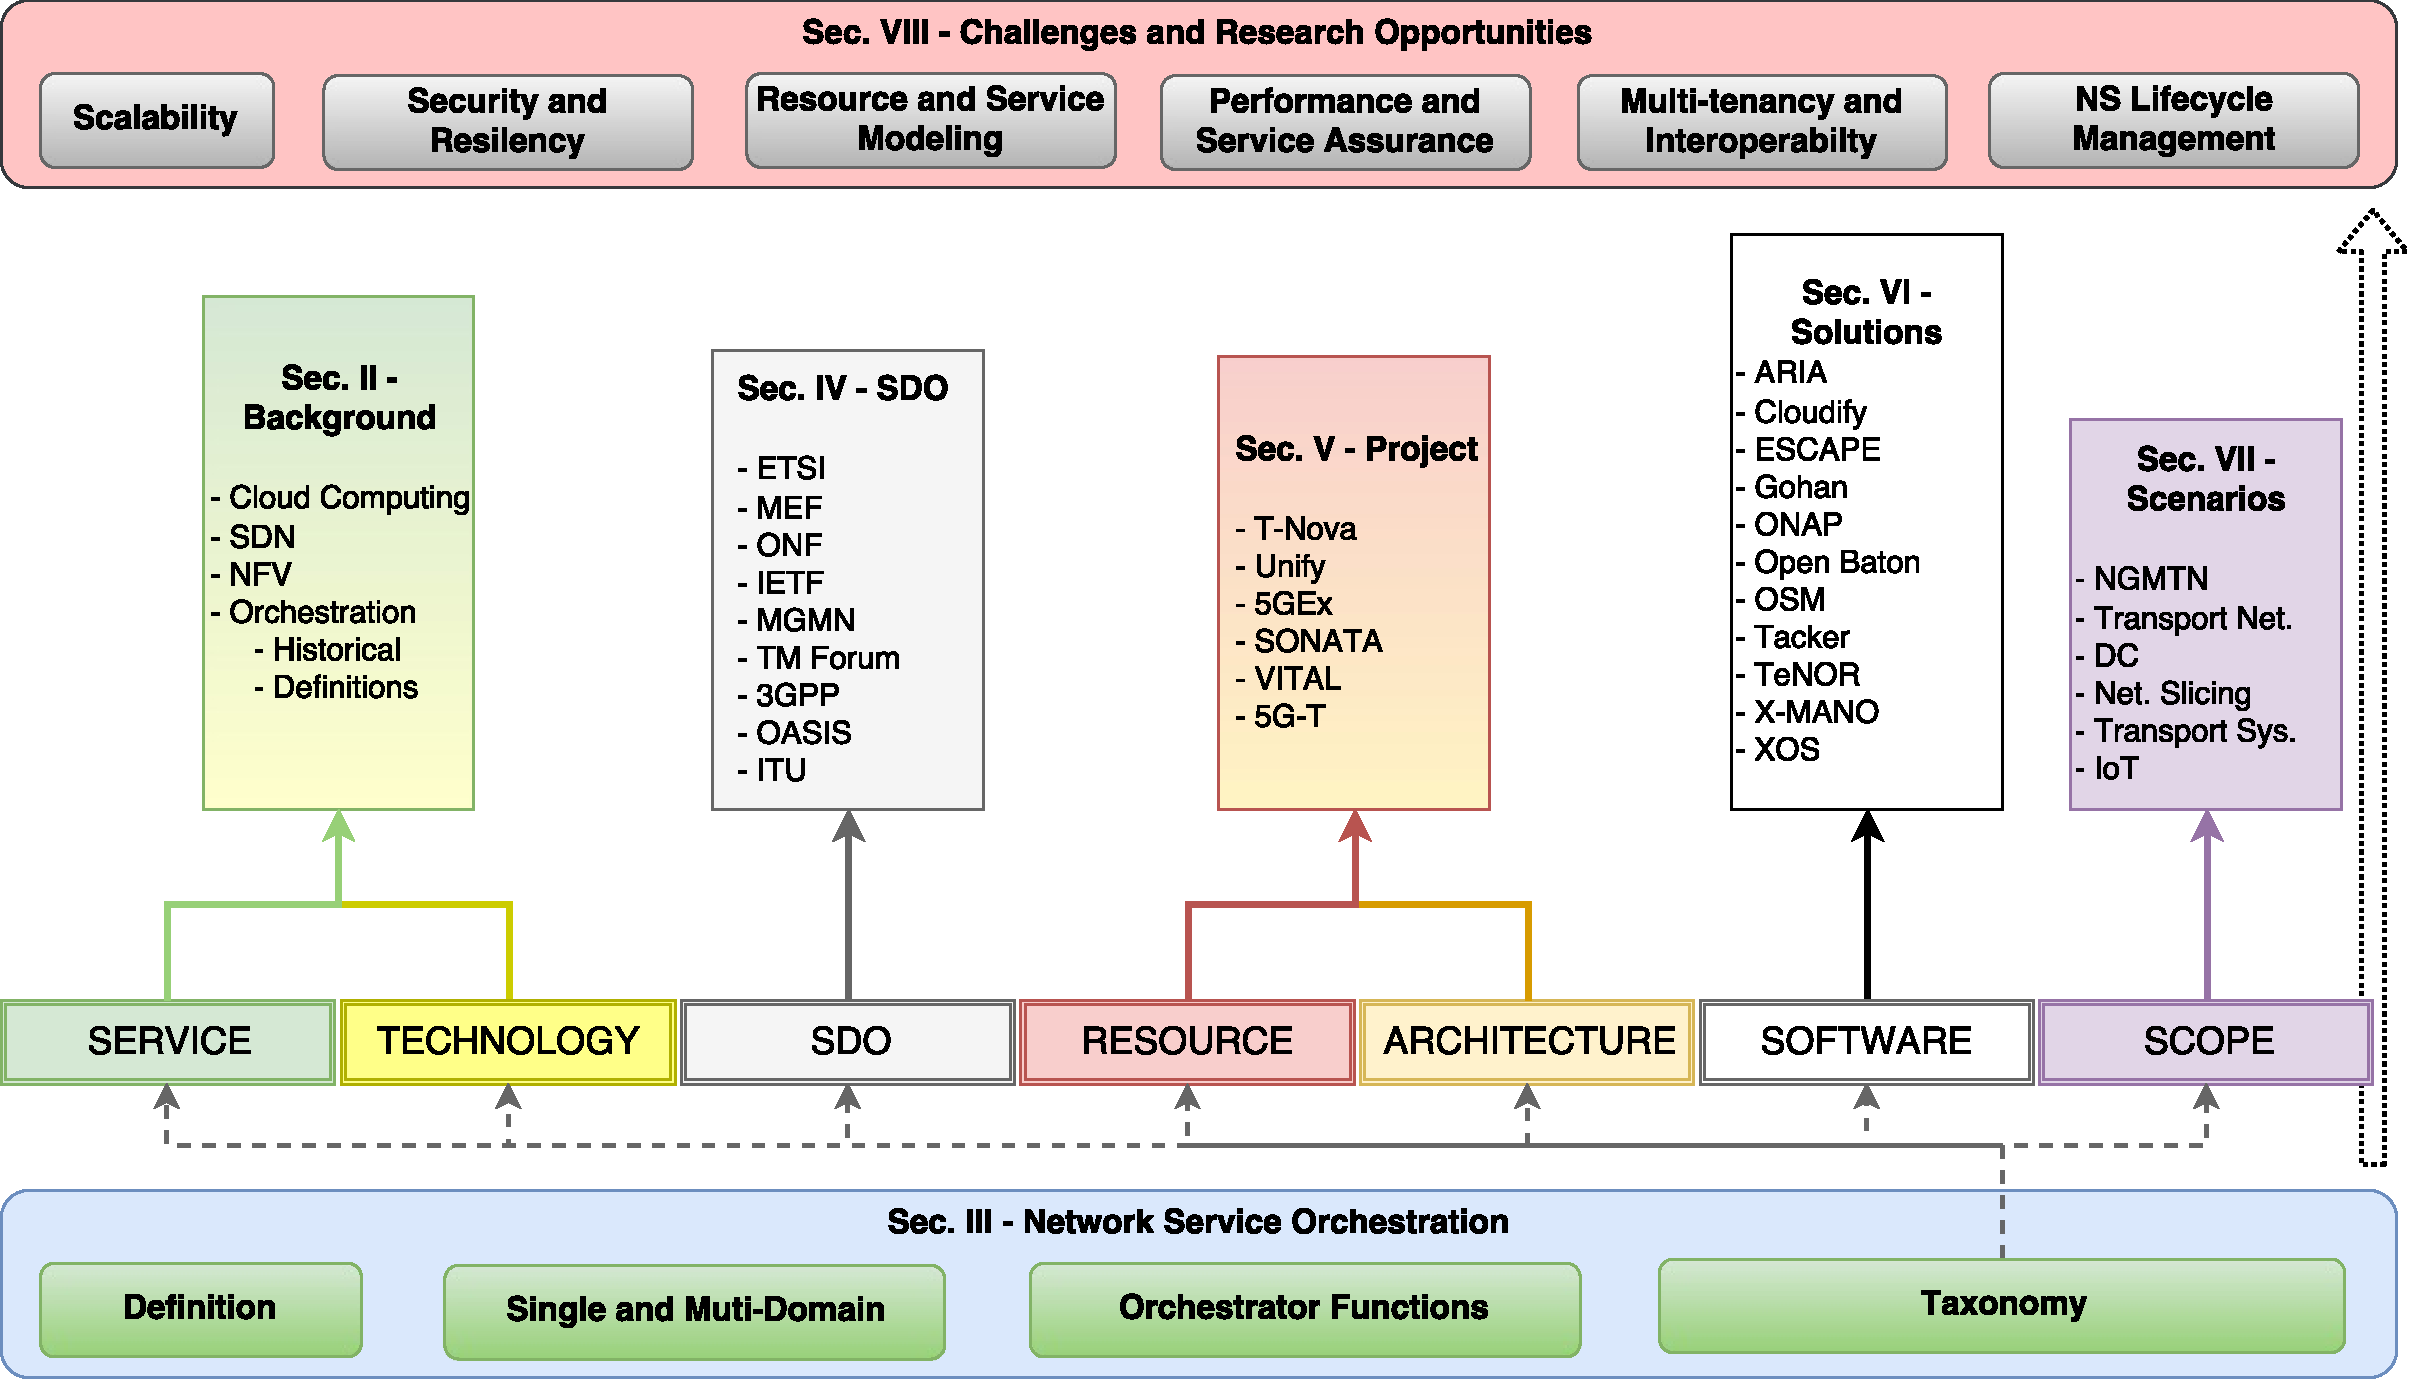
\includegraphics[scale=.4]{Figures/01_Introduction/Organization}
    \caption{Summarized view of this survey on NSO.}
    \label{org}
\end{figure*}

\subsection{Cloud Computing}
Cloud computing is a model for enabling ubiquitous, convenient, on-demand network access to a shared pool of configurable computing resources (e.g., networks, storage, and services) that can be rapidly and automatically provisioned and released with minimal effort~\cite{Mell2011TheTechnology}. Thereby, the resources are traded on demand, that is, the customer only pays what to use. Cloud computing becomes one of relevant technology for the 5G networks mainly because it provides high data rate, high mobility, and centralized management \cite{Le2016SurveyNetworks}.

The service models of cloud computing  are generally categorized into three classes: \gls{saas}, \gls{paas}, and \gls{iaas}. In a cloud \gls{iaas}, the infrastructure is offered as a service to the customer. Each customer can have its virtual resources, such as compute, storage, and network. 
\gls{saas} includes applications such as Facebook, Google Apps, Twitter, and Microsoſt Office 365.

\gls{paas} provides services according to a user’s applications without installing or configuring the operating system. The customers can develop and deploy their applications in the same development environment. The \gls{paas} model includes services such as Microsoft Azure, Google App Engine, RedHat OpenShift, and Amazon Elastic Beanstalk.  

In \gls{saas}, in turn, the customer is able to use the providers' applications running on a cloud infrastructure~\cite{Mijumbi2016NetworkChallenges}. The softwares are maintained and managed by a cloud provider. \gls{iaas} includes applications, for example, OpenStack, CloudStack, Amazon CloudFormation, and Google Compute Engine.

In a cloud environment, the notion of orchestration has also been used for integrating basic services~\cite{Vouk2008CloudImplementations}. The Orchestration in the cloud involves dynamically deploying, managing and maintaining resource and services across multiple heterogeneous cloud platforms in order to meet the needs of clients. This procedure demands to automatize processes and create a workflow. However, this is not a simple task.

\subsection{Software Defined Networking (SDN)}

\gls{sdn}~\cite{surveySDN} is an evolving networking paradigm that attempts to resolve the strongly vertical integration of current network environments. To this end, \gls{sdn} proposals decouple the control plane (i.e. control logic) from the data plane (i.e. data forwarding equipments). With this new architecture, routers and switches become simple forwarding network elements whose control logic is provided by an external entity called \gls{sdn} controller or \gls{nos}. The \gls{sdn} controller creates an abstract network view while hiding details of the underlying physical or virtual infrastructure. Running on the top of the \gls{sdn} controller, software network applications can perform not only traditional functionalities such as routing, load balancing, classification~\cite{6965141}, or \acrlongpl{ids}, but also propose novel use cases such as service  orchestration across multi-domain and multi-technology in 5G networks~\cite{Bernardos20155GInfrastructures}. Those applications together with other industry and academy initiatives towards flexible network services over programmable resources are among the main drivers of \gls{sdn}.

The communication between the \gls{sdn} controller and the forwarding devices is done through \glspl{sbi}, which allow decoupling the control and data plane via open communication protocols (i.e. well-defined APIs). Different \gls{sdn} \glspl{sbi} can be considered (e.g., ForCES~\cite{Doria2010}, OVSDB~\cite{Davie2013RFCProtocol}, POF~\cite{song2013protocol}, etc.), with  OpenFlow~\cite{openFlow},~\cite{SDXCentral2014WhatAPIs} being the most widely accepted solution available in commercial and open source (hardware and software) devices. 

Service orchestrators, OSSes and other network applications can be developed on top of high-level \glspl{nbi} offered by a \gls{sdn} controller. Indeed, \acrshortpl{nbi} are crucial components to control and monitor the network services orchestration. Unlike \acrshortpl{sbi}, where Openflow is a well-known \gls{sdn} standard protocol, \acrshortpl{nbi} are still an open issue with different controllers offering a variety of \acrshortpl{nbi} (e.g., RESTful APIs~\cite{richardson2008restful}, NVP NBAPI~\cite{onix},~\cite{koponen2014network}, SDMN API~\cite{pentikousis2013mobileflow}, etc.). In addition, other type of high-level \acrshortpl{nbi} category are implemented as \gls{nos} management applications~\cite{Rotsos2017NetworkSurvey}. Examples of this category include Virtual Tenant Networks, ALTO, and Intent-based networking (IBN).

The logically centralized \gls{sdn} controller act in spirit of computer operating systems that provide a high-level abstraction for the management of computer resources (e.g., hard drive, CPU, memory) by playing the network operating system role for network management~\cite{gude2008nox}. As such, it provides a set of services (base network services, management, orchestration) and common interfaces (North/South/East/West) to developers who can implement different control applications and improve manageability of networks. Moreover, such interfaces are used within the \gls{mano} framework to deploy end-to-end connectivity. As today, the most popular open source \gls{sdn} controllers are \gls{onos}~\cite{ON.LABONOSScale-out.} and OpendayLight~\cite{LinuxFoundationOpenDaylight}.

In SDN, the concept of orchestration is vital to automate network operations properly. SDN network domains need single-domain or multi-domain orchestration systems to coordinate end-to-end connectivity services through different network domains controlled by different SDN controller instances, which in turn must communicate directly with the physical network~\cite{SDNevolution}.

\subsection{Network Function Virtualization (NFV)}

Traditionally, the telecommunication operators have based their networks on a built-in infrastructure strongly coupled to physical topologies and proprietary devices, resulting in network services constrained to the network topology and the physical location of the network appliances. As a consequence, it becomes hard for providers to offer new services with lower cost and more efficiency and agility \cite{Mijumbi2016NetworkChallenges}. \acrlong{nfv} has been proposed to solve these problems \cite{ETSI2012NetworkAction} and change the mode networks are designed and operated by taking a software-centric approached leveraging advances in virtualization technologies and general purpose processors.

According to \gls{etsi} \gls{isg} \gls{nfv} \cite{ETSIIndustrySpecificationGroupISGNFV2014NetworkNFV},  \acrlong{nfv} is responsible for separating network functions from the hardware and offering them through virtualized services, decomposed into \gls{vnf}, on general purpose servers. With the virtualization of the network functions, \gls{nfv} promises more flexible and faster network function deployment, as well as dynamic scaling of the \glspl{vnf} towards providing finer settings. In \gls{nfv} environment new services do not require new hardware infrastructure, but simply the software installation, i.e. to create \glspl{vnf}.

Moreover, the \gls{nfv} can address \glspl{nf} in the most appropriate location, providing better user traffic performance. The network service can be decomposed in one or more \glspl{vnf}, and each one can be constituted in one or more \glspl{vm}. Each \gls{vnf} is described by a \gls{vnfd} which details the behavioral and deployment information of a \gls{vnf}.

\glspl{vnf} can be connected or combined as building blocks to offer a full-scale network communication service. This connection is known as service chain. Service chain provides logical connectivity between the virtual devices of \gls{nfv} architecture. It is worthwhile noting not only connectivity order importance, but also the logical environment interconnection with physical networks. 

Within the scope of the \gls{isg} \gls{nfv} \cite{ETSIIndustrySpecificationGroupISGNFV2014NetworkNFV}, service chain is defined as a graph of logical links connecting \glspl{nf} towards describing traffic flow between these network functions. This is equivalent to the \gls{sfc}~\cite{Halpern2015} defined by Service Function Chaining Working Group (IETF SFC WG) of the \gls{ietf}.  
An end-to-end network service may cover one or more \gls{nffg} which interconnect \glspl{nf} and end points.  Figure~\ref{nffg} describes two examples of end-to-end network services. The first (green line) is composed of \gls{vcpe} and \gls{vfw} \glspl{vnf} and two endpoints (A1 and A2). The second (red line) is composed of \gls{vcpe} and \gls{vdpi} \glspl{vnf} and two endpoints (B1 and B2). Note that \gls{nfv} allows sharing a multi-tenant \glspl{vnf} between different network services. 

\gls{etsi} has developed a reference architectural framework and specifications in support of NFV management and orchestration. The framework focuses on the support \gls{vnf} operation across different hypervisors and computing resources. It also covers the orchestration and lifecycle management of physical and virtual resources. According to~\cite{ETSIIndustrySpecificationGroupISGNFV2013NetworkFramework}, ``the framework is described at a functional level and it does not propose any specific implementation." Figure~\ref{mano} shows the \gls{etsi} \gls{nfv}-\acrfull{mano} architectural framework with their main functional blocks~\cite{ETSIIndustrySpecificationGroupISGNFV2014NetworkOptions}:

\begin{itemize}
\item Operation/Business Support System (OSS/BSS): block responsible for operation and business applications that network service providers use to provision and operate their network services. It is not tightly integrated into the \gls{nfv}-\gls{mano} architecture.
\item \gls{em}: component responsible for the network management functions FCAPS (Fault, Configuration, Accounting, Performance, and Security) of a running \gls{vnf}.
\item \gls{vnf}: functional block representing the Virtualised Network Function implemented on a physical server. For instance, Router \gls{vnf}, Switch \gls{vnf}, Firewall etc.
\item \gls{nfvi}: representing all the hardware (compute, storage, and networking) and software components where \glspl{vnf} are deployed, managed and executed. 
\item \gls{nfvo}: it is the primary component, in charge of the orchestration of \gls{nfvi} resources across multiple \glspl{vim} and lifecycle management of network services. 
\item \gls{vnfm}: performs configuration and \gls{vnf} lifecycle management (e.g., instantiation, update, query, scaling, termination) on its domain.
\item \gls{vim}: block provides controlling and managing the \gls{nfvi} resources as well the interaction of a \gls{vnf} with hardware resources. For example, OpenStack as cloud platform and OpenDaylight and \gls{onos} as \gls{sdn} controllers.
\end{itemize}

\begin{figure}[t]
  \centering
  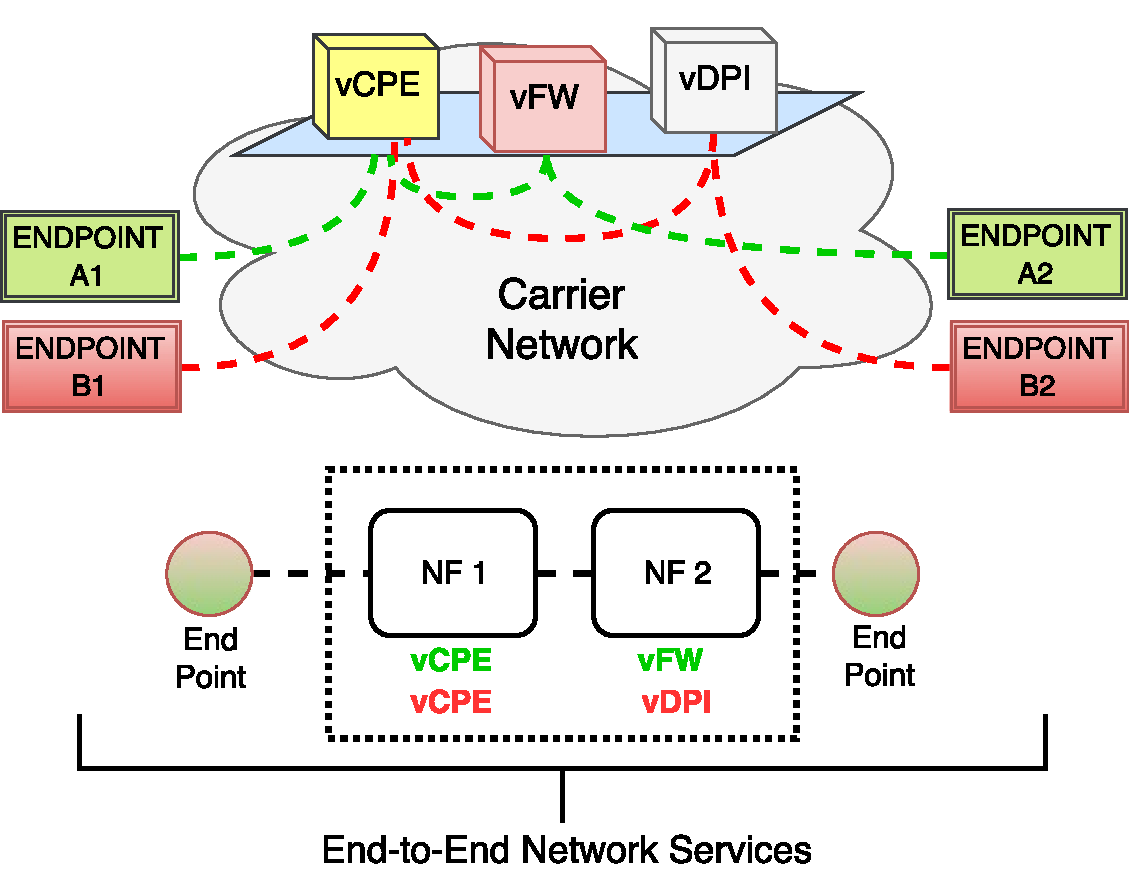
\includegraphics[scale=.45]{Figures/02_Background/ns}
    \caption{Example of two end-to-end network services composed of two \glspl{nf} each. NFV enables the reuse of \glspl{vnf}, e.g., \gls{vcpe}.}
    \label{nffg}
\end{figure}

\begin{figure}[t]
  \centering
  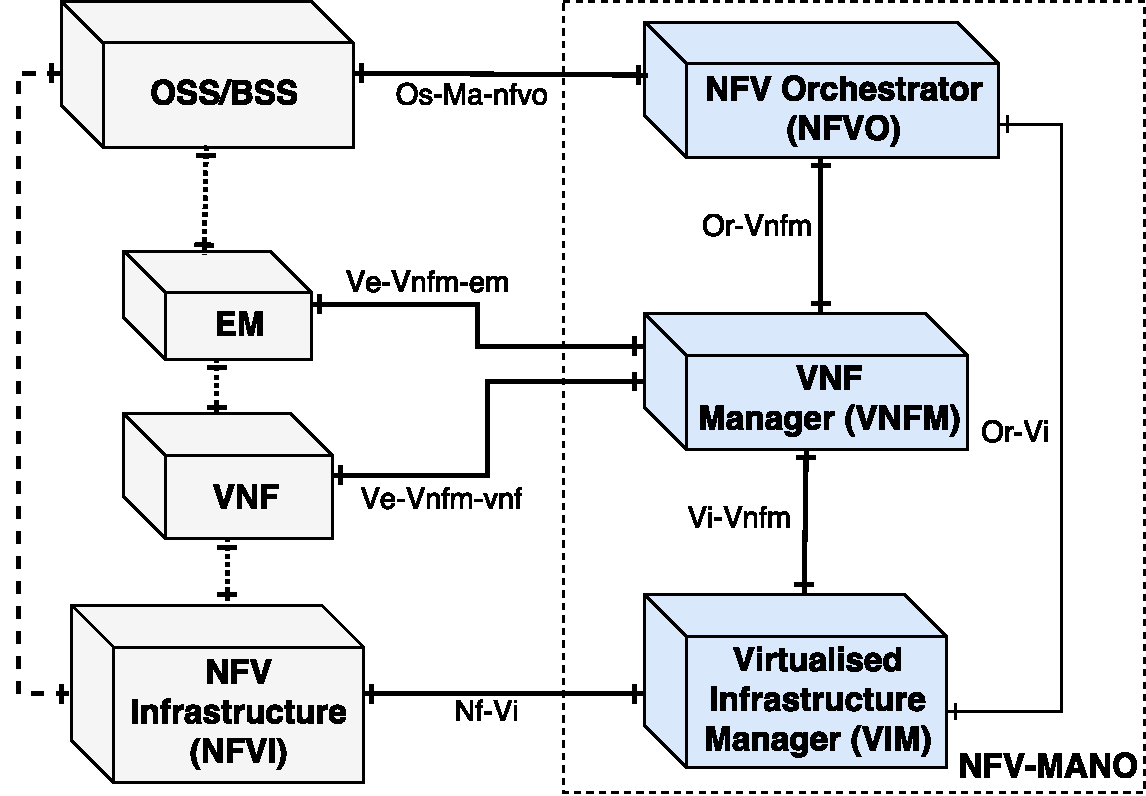
\includegraphics[scale=.4]{Figures/02_Background/MANO}
    \caption{The \gls{nfvmano} architectural framework. Adapted from~\cite{ETSIIndustrySpecificationGroupISGNFV2014NetworkOptions}}
    \label{mano}
\end{figure}

The \gls{nfvmano} functional block performs all the virtualization-specific management, coordination, and automation tasks in the \gls{nfv} architecture including the components \gls{nfvo}, \gls{vnfm}, \gls{vim}, \gls{nfv} Service, \gls{vnf} Catalogue, NFV Instance, and \gls{nfvi} Resource. 

The \gls{nfvmano} reference architecture does not specify anything about \gls{sdn} in its architecture instead it assumes that necessary transport infrastructure is already established and ready to be used. However, in~\cite{ETSINetworkFramework}, \gls{etsi} identifies use cases and the most common options for using SDN in an NFV architectural framework. It also points proof of concepts and recommendations to be fulfilled by the organizations that intend to perform such integration.
\cite{nfv-survey18} provides a recent in-depth survey on NFV state of affairs. 

\subsection{Orchestration: Historical Overview}

The academic community and industry generally require some time to define the real meaning, reach and context of the concepts related to new technology trends as is the case with the term \textit{Orchestration}. 
The term orchestration is used in many different areas, such as multimedia, music, service-oriented architecture, business processes, Cloud, SDN, and, more recently, in NFV.

From an end-user perspective, orchestration reminds a symphony orchestra where a set of instruments play together according to an arrangement. The music is arranged and split in small part, after assigns to different musical instruments. When, who, and what will be played, as well as the conducting are essential parts towards achieving the desired effect.  

One of the first works in the \gls{ict} area that cite the term orchestration \cite{Campbell1992} relate it with coordination and control of multiple media traffics. It distinguishes the orchestration from synchronization and defines an architecture where the orchestration acts in different layers.
In the same scope, \cite{Robbins1997ImplementationArchitecture} relates the orchestration with multimedia data. In this work, the orchestration is associated with multimedia presentation lifecycle management. The lifecycle management involves the coordination of stages that constitute all orchestration process. 

The use of orchestration is also widely discussed in the scope of web services. In this context, orchestration and automation are considered separate processes. The work in \cite{Peltz2003WebChoreography} defines orchestration like an executable process that can interact both internal and external services and must be dynamic, flexible, and adaptable the changes. It emphasizes that orchestration describes how web services can act with each other at the message level, including the business logic and execution order of the activities. 

More recently in 2009, \cite{Galis2009ManagementInternet} provides an overview of definition and design of Management and Service-aware Networking Architectures (MANA) for the \gls{fi}. One of the pillars for the \gls{fi} pointed by the article is Orchestration. In the envisioned architecture, the orchestration function coordinates the integrated behavior and operations to dynamically adapt and optimize resources in response to changing context following business objectives and policies.

Orchestration is generally related to service automation in cloud~\cite{Abosi2011} and \gls{nfv} environments. In spite of that, its concepts are not clearly defined in the scope of \gls{nfv} yet \cite{Kuklinski2016DesignOrchestrators},~\cite{Alvizu2016AdvanceEra}. 

\subsection{Orchestration: Definitions}

Various communities differ with respect to the meaning, assumptions and scope of orchestration functions. Thus, it is helpful begin by reviewing the community understanding to get the main concepts and significance. To this end, we overview the leading organizations and efforts defining the term Orchestration in diverse contexts.

A couple of years ago, the term orchestration was adopted by \gls{etsi} in the scope of \gls{nfv}. In \gls{etsi} \gls{nfv}, the meaning of orchestration is implied, leading to a vague distinction between orchestration and management. Thus, its meaning may just be inferred from the \gls{nfvo} functions (both resources and services layers). Similarly, the Internet Engineering Task Force (\gls{ietf}) comes up with an orchestration definition closely aligned with \gls{etsi}. 

\gls{nist} \cite{Bohn2011NISTArchitecture} was one of the first organizations to define the concept of Service Orchestration. According to NIST vision, orchestration is a process related to the arrangement, coordination, and management of virtualized infrastructure to provide different cloud services to customers.

The \gls{onf} \cite{OpenNetworkingFoundation2016FrameworkNetworks} has formally defined orchestration as usage and selection of resources by orchestrator for satisfying client demands according to the service level. The meaning of the orchestration is evident given a \gls{sdn} Controller. \gls{onf} mentioned that main functions of Orchestration are two-fold. First, orchestration implies to split heavy-loaded service requests into service components. Moreover, it distributes the aforementioned components among supported platforms, creating an integrated end-to-end solution across multiple domains.

The ITU-T Recommendation Y.3300 \cite{InternationalTelecommunicationUnion2014ITU-TNetworking} describes the framework of software defined networking. This recommendation defines that \gls{sdn} functions are programming, orchestrating, controlling and managing network resources. Also, it mentions that orchestration provides automated control and management of network resources. Nevertheless, ITU-T does not clarify the difference between \gls{sdn} functions and orchestration, what causes some confusion.

According to 3GPP Technical Specification 28.801 \cite{3GPP2017TRNetwork}, orchestration is responsible for interpreting and translating a given service request into a configuration of resources (physical and/or virtualized), as needed for service establishment. The configuration of resources may use resource allocation policies or actual available resources. 

In the 5G white paper issued by NGMN \cite{NGMNAlliance2015NGMNPaper}, there is an end-to-end management and orchestration entity which composes the proposed architecture, and it is in charge of translating the service request (business models) into infrastructure resources, beyond managing tasks such as resource scaling and network functions geographic distribution. It is worthwhile noting this proposal is similar to the one presented by \gls{etsi} \gls{nfvo}.  

The \gls{mef}~\cite{MEF:Third:2015} proposes \gls{lso} as a reference architecture for multi-domain orchestration. \gls{lso}, based on network-as-a-service principles, extends the \gls{nfvmano} architecture and creates new capabilities. The orchestration of \gls{lso} refers to "automated service management across multiple operator networks that include fulfillment, control, performance, assurance, usage, security, analytics, and policy capabilities."

In addition to all the above-mentioned leading organizations, there are some works in the literature which also define the concept of orchestration. According to \cite{Rostami2016Multi-Domain5G}, orchestration enables programmability for creating and deploying of end-to-end network services and dynamic network control through a single interface. Thyagaturu et al. \cite{Thyagaturu2016SoftwareSurvey} address orchestration as the coordination of network services and operations in a higher layer, abstracting the underlying physical infrastructure. The work in \cite{Guerzoni2016Multi-domainApproach} makes a generic definition of orchestration as automated management of complex systems and services.

From the definitions of orchestration presented, we can derive a clear relationship among orchestration, automation, and management. Although the three terms are lumped together, it is necessary an understanding  of the differences between them as they are not the same thing. 
Automation describes a simple and technical task without the human intervention, for example, launching a web server, stopping a server. 
Management is responsible for maintaining and healthiness of infrastructure. Its role consists of activities such as alarms for event detection, monitoring, backups of critical systems, upgrades, and license management. 
Orchestration, in turn, is concerned with the execution of a workflow (processes) in a correct order. It controls the overall workflow process from starting the service until it ends. Its objective is to optimize and automate the network service deployment. 

Figure~\ref{diff} illustrates  the relationship among the three terms cited. There is a certain hierarchic between them. The orchestration is a high-level plane, below the management, and in the bottom the automation. In our vision, the orchestration depends on tasks performed by management. Both management and orchestration are based on the use of automation in the execution of their tasks. Nevertheless, some activities are only performed by a certain function, optimization, for instance, can not be achieved by simple automation. The optimization is a responsibility of orchestration. There is a difference between them, but, if they work together in the execution of processes, the services deployments will succeed with further accuracy.